\lstset{style=fsharpstyle}

\section{Анализ требований к программному средству}

\subsection{Используемые технологии}
\label{sec:practice:technology_used}

Выбор технологий является важным предварительным этапом разработки сложных информационных систем.
Платформа и язык программирования, на котором будет реализована система, заслуживает большого внимания, так как исследования показали, что выбор языка программирования влияет на производительность труда программистов и качество создаваемого ими кода.

Ниже перечислены некоторые факторы, повлиявшие на выбор технологий:
\begin{itemize}
\item разрабатываемое ПО должно иметь возможность запускаться под платформами Windows(7,8,10) и Linux(Ubuntu, Arch Linux, Linux Mint);
\item ПО работает в совокупности с другими средствами описания аппарутры интегральных схем и должно иметь возможность запускаться в форме скрипта;
\item среди различных платформ разработки имеющийся программист лучше всего знаком с разработкой на платформе;
\item дальнейшей поддержкой проекта, возможно, будут заниматься разработчики, не принимавшие участие в выпуске первой версии;
\item имеющийся разработчик имеет опыт работы с объекто-ориентированными языками программирования;
\end{itemize}

Основываясь на опыте работы имеющихся программистов разрабатывать ПО целесообразно с помощью языка Java.
Приняв во внимание необходимость обеспечения доступности дальнейшей поддержки ПО, возможно, другой командой программистов, необходимость работы с различными ОС, скриптообразный характер ПО, целесообразно не использовать малоизвестные и сложные языки программирования.

С учетом этого фактора выбор языков программирования сужается до четырех: Python, Ruby и Java. Слабые по сравнению с другими языками механизмы ООП (отсутствие наследования, классов) языка LUA, которые могут быть полезны при разработке ПО, позволяют исключить этот язык из списка кандидатов. Python уступает по удобству использования двум другим кандидатам из нашего списка. Оставшиеся два языка программирования Ruby и Java являются хорошими кандидатами . Тот факт, что Java существует на рынке уже давно, делает этот язык предпочтительным кандидатом.

Таким образом, с учетом вышеперечисленных факторов, целесообразно остановить выбор на следующих технологиях:
\begin{itemize}
  \item операционные системы: семейство Windows(7,8,10), семейство Linux(Ubuntu, Debian, Arch Linux), Mac os;
  \item база данных MySql для хранения информации;
  \item язык программирования Java на котором будет реализована серверная часть программного средства;
  \item язык программирования Javascript и библиотека react js;
\end{itemize}
При реализации программного средства встает вопрос, в каком виде должна храниться вся информация и с помощью каких средств её следует обрабатывать. Так как, например, информация о каждом отдельном объявлении представляет собой типичный набор данных (площадь, количество комнат, этаж, год постройки и т. д.), то очевидно, что в этом случае целесообразно хранить их в реляционной базе данных на сервере. Посредством запросов к базе данных пользователь может получать нужные ему сведения, а администратор может добавлять и изменять данные. Выбор конкретной СУБД в качестве сервера баз данных осуществлялся исходя из тех преимуществ, которые она имеет перед другими, а также удобства работы с ней. В данном случае был выбрана клиент-серверная СУБД MySQL

Для реализации поставленной задачи предпочительно использовать на ранних этапах базу данных MySql. В случаи большого количество информации, можно будет слегкость мигрировать на другую СУБД, т.к язык Java использует спецификацию JPA, которая позволяет с легкостью мигрировать на другую СУБД.

Объектно-ориентированный язык программирования Java широко используется для создания серверных приложений. Язык java будет использован для создания высокоуровнего дизайна проложения (иерархия классов и интерфейсов, организация модулей и публичного программного интерфейса), реализации логики приложения, функций и методов~\cite{dpir_2007}, прототипирования различных идей.

Для реализации клиентской части был выбран язык программирования Javascript. Для быстроты и удобства реализации, будет использована библиотека react.js, которая написана на языке программирования Javascript. 


\subsubsection{Язык программирования Java}
\label{sub:practice:ruby_overview}
Объектно-ориентированный язык программирования Java широко используется для создания серверных приложений.

Система Java создана на основе простого языка программирования, техника использования которого близка к общепринятой и обучение которому не требует значительных усилий.

Java как язык программирования является объектно-ориентированным с момента основания. Кроме того программист с самого начала обеспечивается набором стандартных библиотек, обеспечивающих функциональность от стандартного ввода/вывода и сетевых протоколов до графических пользовательских интерфейсов. Эти библиотеки легко могут быть расширены.

Несмотря на то, что язык С++ был отвергнут, синтаксис языка Java максимально приближен к синтаксису С++. Это делает язык знакомым широкому кругу программистов. В то же время из языка были удалены многие свойства, которые делают С++ излишне сложным для пользования, не являясь абсолютно необходимыми. В результате язык Java получился более простым и органичным, чем С++.

Надежность и безопасность Java существенно облегчает создание надежного программного обеспечения. Кроме исчерпывающей проверки на этапе компиляции, система предусматривается анализ на этапе выполнения. Сам язык спроектирован так, чтобы вырабатывать у программиста привычку писать "правильно". Модель работы с памятью, в которой исключено использование указателей, делает невозможными целый класс ошибок, характерных для С и С++.

В силу того, что Java предназначен для работы в распределенной среде, безопасность становится чрезвычайно важной проблемой. Требования безопасности определяют многие черты как языка, так и реализации всей системы.
Компилятор Java производит байт-коды, т.е. модули приложения имеют архитектурно-независимый формат, который может быть проинтерпретирован на множестве разнообразных платформ. Это уже не исходные тексты, но еще не платформно-зависимые машинные коды.

Схема работы системы и набор байт-кодов виртуальной машины Java таковы, что позволяют достичь высокой производительности на этапе выполнения программы:

анализ кодов на соблюдение правил безопасности производится один раз до запуска кодов на выполнение, в момент выполнения таких проверок уже не нужно, и коды выполняются максимально эффективно ;

работа с базовыми типами максимально эффективна, для операций с ними зарезервированы специальные байт-коды;

методы в классах не обязательно связываются динамически;

автоматический сборщик мусора работает отдельным фоновым потоком, не замедляя основную работу программы, но в то же время обеспечивая своевременный возврат свободной памяти в систему;

стандарт предусматривает возможность написания критических по производительности участков программы в машинных кодах;

Каждая из перечисленных характеристик по отдельности может быть найдена в уже существующих программных пакетах. Новым является соединение их в стройную непротиворечивую систему, которая должна стать всеобщим стандартом.

Java полагается на автоматическое управление памятью со стороны исполняющей среды, предоставляя совсем немного средств для управления жизненным циклом объектов.
Не смотря на это, в языке все же присутствуют указатели на функции.

Создатели языка Java не являются противниками привнесения в язык новых идей и возможностей.
Каждая новая версия интерпретатора языка привносит различные полезные возможности, которые отвечают требованиям индустрии.


\subsubsection{Система управления базами данных MySQL}
\label{sub:practice:vhdl_overview}
Выбор конкретной СУБД в качестве сервера баз данных осуществлялся исходя из тех преимуществ, которые она имеет перед другими, а также удобства работы с ней. В данном случае был выбрана клиент-серверная СУБД MySQL. Её архитектура изображена на рисунке ниже. 

\begin{figure}[!htb]
	\centering
	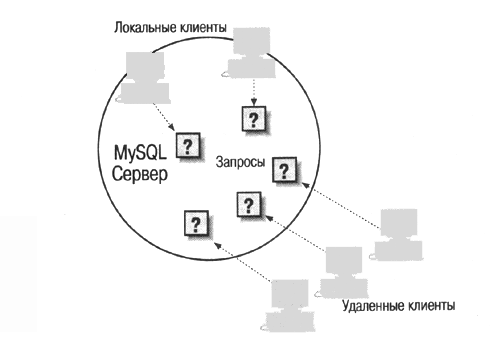
\includegraphics[scale=0.5]{mysql.png}
	\caption{ Клиент-серверная архитектура MySQL}
	\label{fig:arch_and_mod::lexer_flow}
	\clearpage
\end{figure}

Клиент-серверная архитектура MySQL
Самая подходящая для MySQL сфера применения - это Интернет, благодаря хорошей системе безопасности этого пакета, стабильной работе и высокому быстродействию. Для создания скриптов был выбран язык программирования PHP, а MySQL – самая популярная СУБД, которая поддерживается этим языком. В PHP есть множество функций, которые позволяют удобно и эффективно работать с базами данных – и это одна из причин выбора данной СУБД.

Рассмотрим преимущества MySQL:

\begin{itemize}

	\item Быстродействие. Благодаря внутреннему механизму многопоточности быстродействие MySQL весьма высоко. Для разработчиков MySQL скорость всегда являлась ключевым параметром. Новые возможности добавлялись в пакет MySQL только после того, как их удавалось реализовать без ущерба для производительности. Иногда это означало, что некоторые возможности добавлялись не так быстро, как хотелось бы пользователям, но зато всегда гарантировало быструю работу MySQL.

	\item Безопасность. Довольно высокий уровень безопасности обеспечивается благодаря базе данных mysql, создающейся при установке пакета и содержащей пять таблиц. При помощи этих таблиц можно описать, какой пользователь из какого домена с какой таблицей может работать и какие команды он может применять. Пароли, хранящиеся в базе данных, можно зашифровать при помощи встроенной в MySQL функции password().

	\item Лицензия.Раньше лицензирование MySQL было немного запутанным; сейчас эта программа для некоммерческих целей распространяется бесплатно.

	\item Открытость кода. Благодаря этому программист может сам добавлять в пакет нужные функции, расширяя его функциональность так, как ему требуется. За отдельную плату это могут сделать и сами авторы MySQL. 

	\item Простота использования. Для начала работы с MySQL не требуется сложной процедуры конфигурации. MySQL Server начнёт работать соответствующим образом сразу. По умолчанию выбираются значения, соответствующие минимальному использованию ресурсов диска и памяти. Для получения оптимальной производительности и для специальных условий (например, для проверки входа в систему), конечно же, потребуется дополнительная настройка. Чтобы помочь выполнить такую настройку, предлагаются соответствующие примеры файлов типовой конфигурации.

	\item Сообщество. Как следствие открытости кода, бесплатности программы, стабильной и надежной ее работы образовалось сообщество людей, которые не просто лояльны к MySQL, но и всячески участвуют как в развитии самого пакета, так и в обучении менее опытных людей работе с ним. Существует огромное количество листов рассылки и конференций, где можно получить бесплатную помощь в любое время суток.
\end{itemize}

В настоящее время существуют версии программы для большинства распространенных компьютерных платформ. Это говорит о том, что вам не навязывают определенную операционную систему. Вы сами можете выбрать, с чем работать, например с Linux или Windows, но даже в случае замены ОС вы не потеряете свои данные и вам даже не понадобятся дополнительные инструменты для их переноса.
Конечно же, как и любое программное средство, СУБД MySQL не избавлена от некоторых недостатков. Например, можно назвать отсутствие вложенных запросов, что приводит к необходимости находить нужные значения отдельно и подставлять их в другой запрос непосредственно в CGI-сценарии, что, несомненно, сказывается на производительности.
Несмотря на это, СУБД MySQL была выбрана как наиболее подходящий сервер баз данных для программного средства.

\subsubsection{Язык программирования Javascript}

JavaScript — прототипно-ориентированный сценарный язык программирования. Является реализацией языка ECMAScript (стандарт ECMA-262).

JavaScript обычно используется как встраиваемый язык для программного доступа к объектам приложений. Наиболее широкое применение находит в браузерах как язык сценариев для придания интерактивности веб-страницам.

Основные архитектурные черты: динамическая типизация, слабая типизация, автоматическое управление памятью, прототипное программирование, функции как объекты первого класса.

Структурно JavaScript можно представить в виде объединения трёх чётко различимых друг от друга частей:

\begin{itemize}
	\item ядро (ECMAScript),
	\item объектная модель браузера (Browser Object Model или BOM (en)),
	\item объектная модель документа (Document Object Model или DOM).
\end{itemize}

Если рассматривать JavaScript в отличных от браузера окружениях, то объектная модель браузера и объектная модель документа могут не поддерживаться.

Объектную модель документа иногда рассматривают как отдельную от JavaScript сущность, что согласуется с определением DOM как независимого от языка интерфейса документа. В противоположность этому ряд авторов находят BOM и DOM тесно взаимосвязанными.

На JavaScript оказали влияние многие языки, при разработке была цель сделать язык похожим на Java, но при этом лёгким для использования непрограммистами. Языком JavaScript не владеет какая-либо компания или организация, что отличает его от ряда языков программирования, используемых в веб-разработке.

JavaScript является объектно-ориентированным языком, но используемое в языке прототипирование обуславливает отличия в работе с объектами по сравнению с традиционными класс-ориентированными языками. Кроме того, JavaScript имеет ряд свойств, присущих функциональным языкам — функции как объекты первого класса, объекты как списки, карринг, анонимные функции, замыкания — что придаёт языку дополнительную гибкость.

Несмотря на схожий с Си синтаксис, JavaScript по сравнению с языком Си имеет коренные отличия:

\begin{itemize}
	\item объекты, с возможностью интроспекции;
	\item функции как объекты первого класса;
	\item автоматическое приведение типов;
	\item автоматическая сборка мусора;
	\item анонимные функции;
\end{itemize}

В языке отсутствуют такие полезные вещи, как:

\begin{itemize}
	\item JavaScript не предоставляет возможности управлять зависимостями и изоляцией областей видимости;
	\item отсутствует интерфейс программирования приложений по работе с файловой системой, управлению потоками ввода-вывода, базовых типов для бинарных данных;
	\item стандартные интерфейсы к веб-серверам и базам данных;
	\item система управления пакетами которая бы отслеживала зависимости и автоматически устанавливала их;
\end{itemize}

React является библиотекой, написаной на JavaScript с открытым исходным кодом для создания пользовательских интерфейсов. Библиотека была написана разработчиками из Facebook, Instagram и сообществом индивидуальных разработчиков и корпораций. 

React позволяет разработчикам создавать крупные веб-приложения, которые используют данные, которые могут меняться со временем, без перезагрузки страницы. Его основная цель - быть быстрым, простым и масштабируемым. 

Клиентская часть программного средства, будет разработана с помощью языка Javascript и библиотеки Ract.

\subsection{Функциональное моделирование}

Для функционального моделирования программного средства для продажи квартир использована диаграмма вариантов использования, являющаяся частью унифицированного языка моделирования (UML).
Общий вид обобщенной диаграммы вариантов использования удаленного управления мультимедиа представлен ниже.

\begin{figure}[!htb]
	\centering
	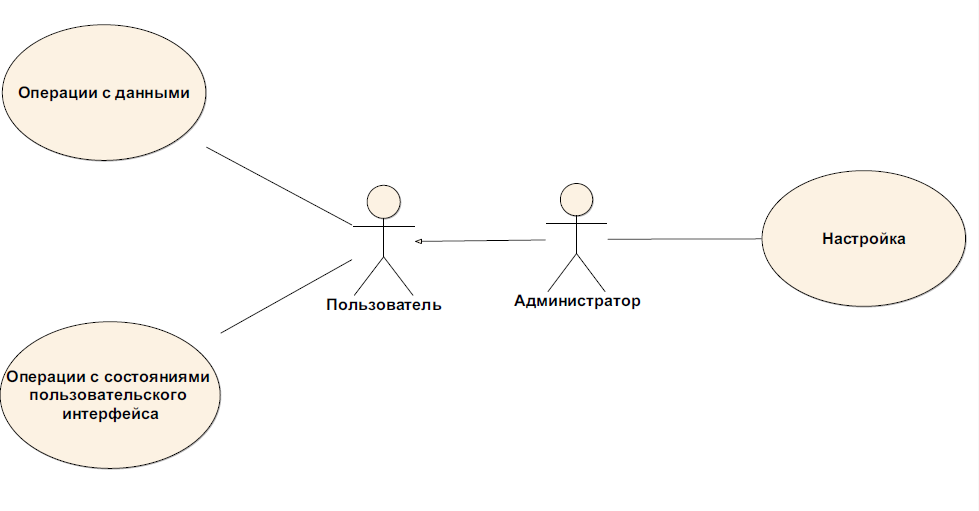
\includegraphics[scale=0.5]{general_use_case.png}
	\caption{ Диаграмма вариантов использования}
	\label{fig:arch_and_mod::lexer_flow}
	\clearpage
\end{figure}

Как видно из диаграммы, для программного средства необходимы два актера:

\begin{itemize}
	\item пользователь – это любой конечный пользователь из круга лиц, имеющий доступ к удаленному управлению данными на устройствах;
	\item администратор – это такой пользователь, который кроме всех обычных функций, доступных пользователю, имеет еще специфические функции настройки данных; следует отметить, что администратор наследуются от пользователя.
\end{itemize}

Среди основных функций пользователя можно выделить:

\begin{itemize}
	\item операции с данными: все функции, связанные с отображением и управлением мультимедийных данных, дополнительные специфические функции с мультимедиа;
	\item операции с состояниями пользовательского интерфейса: все функ-ции, предназначенные для управления состояниями пользовательского ин-терфейса.
\end{itemize}

У администратора следует выделить функции настройки программного средства, предназначенные настройки всех компонент, связанных с коректной работой пользователя.

Рассмотрим необходимые функции для работы с объявлениями. диаграмма вариантов использования «Работа с объявлениями» представлена ниже.

\begin{figure}[!htb]
	\centering
	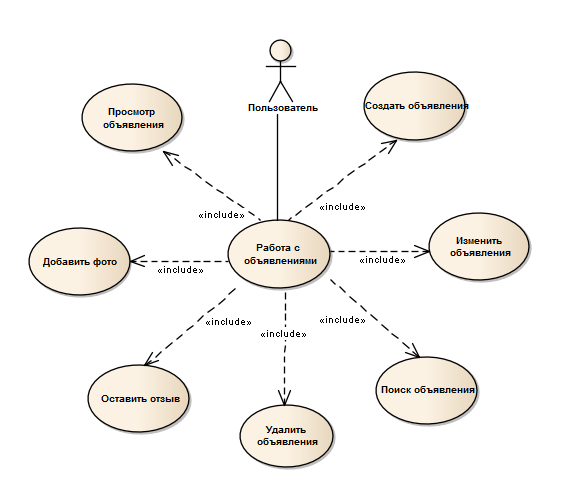
\includegraphics[scale=0.8]{notes_use_case.png}
	\caption{ диаграмма вариантов использования «Работа с объявлениями»}
	\label{fig:arch_and_mod::lexer_flow}
	\clearpage
\end{figure}

Как видно из диаграммы, функция «Работа с объявлениями» включает в себя следующие возможности:

\begin{itemize}
	\item «Создать объявления»: данная функция дает возможность пользователю создавать объявления для возможности выставить свою недвижимость на продажу. 
	\item «Изменить объявление»: функция означает возможность пользователем изменять ранее созданные объявления. Включает возможность редактирования информация, которая была описана при создании объявления.
	\item «Поиск объявления»: такая функция означает возможность пользователя поиска объявления для покупки или аренды недвижимости. Данная функция включает в себя множество критериев для поиска.
	\item «Удалить объявления»: функция означает возможность удалить выбранное объявление.
	\item «Оставить отзыв»: функция дает возможность пользователем добавлять комментарии, задавать дополнительные вопросы на счет недвижимости.
	\item «Добавить фото»: функция означает возможность пользователю добавить фото о недвижимости.
	\item «Просмотр объявления»: функция дает возможность пользователям просматривать объявление о недвижимости.
\end{itemize}

Рассмотрим подробнее функцию «Создать новое объявление». Диаграмма вариантов использования представлена ниже.


\begin{figure}[!htb]
	\centering
	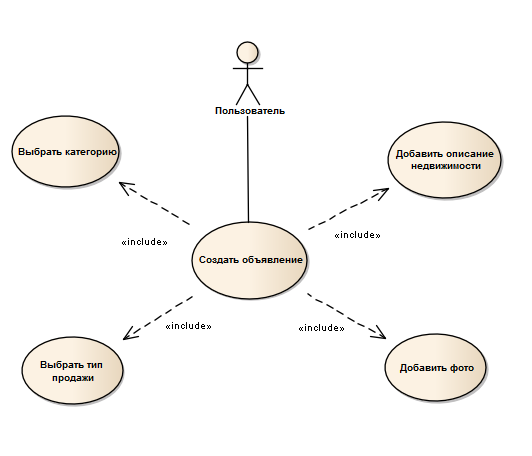
\includegraphics[scale=0.8]{create_note_use_case.png}
	\caption{ Диаграмма вариантов использования «Создать объявление»}
	\label{fig:arch_and_mod::lexer_flow}
	\clearpage
\end{figure}

Как видно из диаграммы, функция «Создать объявления» включает в себя следующие возможности:

\begin{itemize}
	\item «Добавить описание недвижимости»: данная функция дает возможность пользователю добавить необходимую информацию о своей недвижимости. Данная информация будет видна другим пользователям.  
	\item «Добавить фото»: функция означает возможность пользователю добавить фотографии о недвижимости. Например пользователь может добавить фотографию планировки квартиры, фотографию гостиной, фотографию кухни и т.д .
	\item «Выбрать тип продажи»: эта функция дает возможность пользователя выбрать тип продажи недвижимости. Будет это аренда жилья, чистая продажа недвижимости или обмен с доплатой.
	\item «Выбрать категорию»: эта функция дает возможность пользователя выбрать категорию объявления. В зависимости от категории, будущее объявление будет размещено в нужной секции. Это функция облегчает поиск для других клиентов.
\end{itemize}

Рассмотрим необходимые функции для роли «Администратор». Диаграмма вариантов использования представлена ниже.

\begin{figure}[!htb]
	\centering
	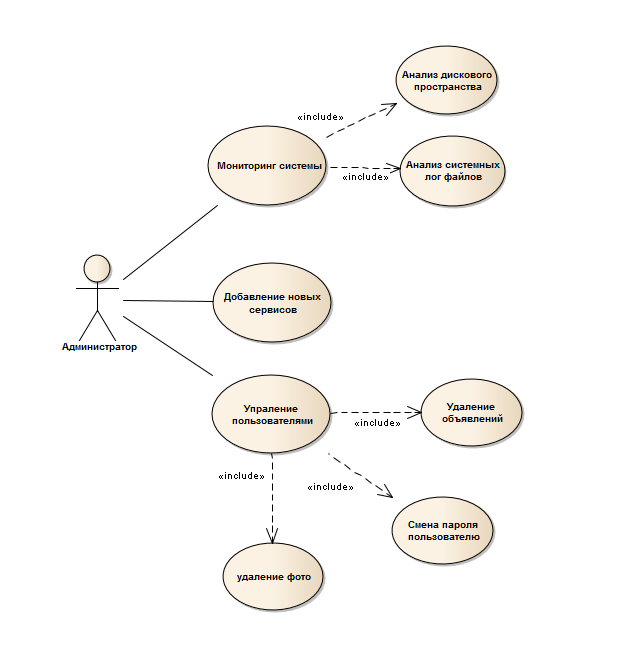
\includegraphics[scale=0.8]{admin_use_case.png}
	\caption{ Диаграмма вариантов использования для роли «Администратор»}
	\label{fig:arch_and_mod::lexer_flow}
	\clearpage
\end{figure}

Данная диаграмма показывает, какими функциями должен обладать пользователь, с ролью администратор.  Рассмотрим каждую функции в подробном описании:

\begin{itemize}
	\item «Анализ дискового пространства»: данная функция дает возможность администратору смотреть свободное место дискового пространства. Данная функция необходима, чтобы периодически чистить устаревшую информацию, которая будет храниться на диске.
	\item «Анализ системных лог файлов»: функция означает возможность администратору просматривать системные лог файлы на наличие ошибок. В случаи сбоя приложения, пользователю необходима узнать по какой причине произошёл сбой. 
	\item «Добавление новых сервисов»: эта функция дает возможность администратору добавить новый сервис. данная функция предназначена для расширения функционала будущего программного средства. 
	\item «Удаление объявления»: эта функция дает возможность администратору удалить любое объявление. Данная функция предназначена для удаления устаревших и неактуальных объявлений, в случаи, если пользователь сам не удалил объявление.
	\item «Удаление фото»: эта функция дает возможность администратору удалить любые фотграфии. Данная функция предназначена для удаления устаревших и неактуальных фотографий в случаи, если пользователь сам не удалил объявление.
	\item «Смена пароля пользователю»: функция дает возможность администратору сменить пароль пользователю. Например, если пользователь не смог восстановить пароль с помощью стандартных методов, он может обратиться в сервисный центр.
\end{itemize}

Для возможности пользоваться программным средством, необходима учётная запись.  

Учётная запись это хранимая в компьютерной системе совокупность данных о пользователе, необходимая для его опознавания (аутентификации) и предоставления доступа к его личным данным и настройкам. Учётная запись, как правило, содержит сведения, необходимые для опознания пользователя при подключении к системе, сведения для авторизации и учёта. Это идентификатор пользователя (login) и его пароль. Пароль, как правило, хранится в зашифрованном или хэшированном виде для обеспечения его безопасности. Для использования учётной записи (другими словами, для входа в систему под чьим-то именем) необходимо использовать логин и пароля. Для регистрации необходимо использовать дополнительное поле email. 

Рассмотрим необходимые функции для работы с учетной записью. Данная диаграмма показывает, что пользователь может делать с учетной записью. 

Диаграмма вариантов использования представлена ниже.

\begin{figure}[!htb]
	\centering
	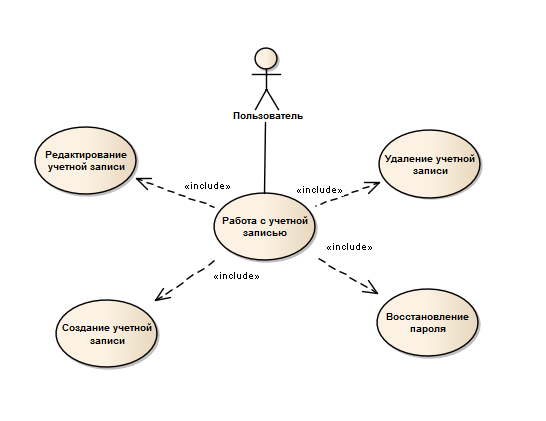
\includegraphics[scale=0.8]{account_use_case.png}
	\caption{ Диаграмма вариантов использования «Работа с учетной записью»}
	\label{fig:arch_and_mod::lexer_flow}
	\clearpage
\end{figure}

Рассмотрим каждую функцию подробнее:

\begin{itemize}
	\item «Создание учетной записи»: данная функция дает возможность пользователю завести учетную запись, чтобы использовать возможности программного средства.
	\item «Редактирование учетной записи»: данная функция позволяет пользователю изменить или дополнить информацией свою учетную запись.
	\item «Удаление учетной записи»: данная функция позволяет пользователю удалить свою учетную запись.
	\item «Восстановление пароля»: данная функция дает возможность пользователю востановить пароль от учетной записи. 
\end{itemize}

\subsection{Разработка спецификации функциональных требований}

На основе функциональной модели ПС и поставленных задач необходимо разработать спецификацию функциональных требований к программному средству для продажи квартир.

Спецификация функционального требования «Создание учетной записи пользователя»:

\begin{itemize}
	\item Функции создания учетной записи должна быть доступна только клиентам;
	\item При нажатии пользователем на кнопку «sign up» на экране отображается окно, в котором пользователь должен указать логин, пароль, электронную почту;
	\item  После нажатия на кнопку “create” в системе должен появиться новый пользователь. Должно произойти перенаправление на страницу входа в программное средство; 
	\item Если логин или электронная почта уже используется у другого пользователя, ПС должно предложить пользователю ввести другой логин и электронную почту, т.к такие данные уже используются;
\end{itemize}

Спецификация функционального требования «Восстановление учетной записи пользователя»:

\begin{itemize}
	\item Функции должна быть доступна только клиентам;
	\item При нажатии пользователем на кнопку «forgot password» на экране отображается окно, в котором пользователь должен указать свою  электронную почту для восстановления пароля;
	\item После нажатия на кнопку “restore” на почту должны прийти инструкции как восстановить пароль. Должно произойти перенаправление на страницу входа в программное средство; 
\end{itemize}


Спецификация функционального требования «Добавление объявления»:

\begin{itemize}
	\item Функции должна быть доступна только клиентам;
	\item При нажатии пользователем на кнопку «forgot password» на экране отображается окно, в котором пользователь должен указать свою  электронную почту для восстановления пароля;
	\item  После нажатия на кнопку “restore” на почту должны прийти инструкции как восстановить пароль. Должно произойти перенаправление на страницу входа в программное средство;
\end{itemize}

Спецификация функционального требования «редактирование объявления»:

\begin{itemize}
	\item Функции должна быть доступна только клиентам;
	\item Функция редактирования мультимедиа должна быть доступна, после выбора файла и отмечена галочкой;
	\item Нажатие пользователем во время редактирования клавиши «Cancel» должно отменить редактирование;
	\item При нажатии пользователем во время редактирования на клавишу «Enter» редактируемое мультимедиа должно быть сохранено;
	\item После редактирования выбранного мультимедиа страница должна быть обновлена;
\end{itemize}

Спецификация функционального требования «удаления  объявления»:

\begin{itemize}
	\item Функции должна быть доступна всем;
	\item При нажатии пользователем на кнопку удаления должно быть показано окно с подтверждением удаления; 
	\item После удаления выбранного мультимедиа страница должна быть обновлена;
\end{itemize}

Спецификация функционального требования «добавление фотографий»:

\begin{itemize}
	\item Функции должна быть доступна только клиентам;
	\item на странице объявления должна присутствовать кнопка «Add photo». При нажатии на кнопку,  появляется диалоговое окно;
	\item в диалоговом окне должны быть кнопки «choose photo», «add», «cancel»;
	\item при нажатии кнопки «choose photo» пользователь должен выбрать фото;
	\item после нажатия кнопки «Add» выбранная фотография появляется на странице объявления;
	\item при нажатии кнопки «cancel» происходит отмена данной операции;
\end{itemize}

Спецификация функционального требования «поиск объявления»:

\begin{itemize}
	\item Функции должна быть доступна только клиентам;
	\item На главной странице должна присутствовать панель для поиска объявлений;
	\item На панели должны быть следующие критерии для поиска: ценовой диапазон, город, район, количество комнат, типа продажи, тип категории, кнопка «Search»;
	\item При нажатии на кнопку «Search» в центре экрана появляются найденные объявления;
\end{itemize}

Спецификация функционального требования «Добавления отзывы»:

\begin{itemize}
	\item Функции должна быть доступна только клиентам;
	\item на странице объявления должна присутствовать кнопка «Add comment». При нажатии на кнопку, появляется диалоговое окно;
	\item после нажатия кнопки «Add» отзыв появляется на странице объявления;
\end{itemize}

